%% LaTeX-Beamer template for KIT design
%% by Erik Burger, Christian Hammer
%% title picture by Klaus Krogmann
%%
%% version 2.1
%%
%% mostly compatible to KIT corporate design v2.0
%% http://intranet.kit.edu/gestaltungsrichtlinien.php
%%
%% Problems, bugs and comments to
%% burger@kit.edu
\pdfminorversion=4

\documentclass[18pt]{beamer}

\usepackage[utf8]{inputenc}
\usepackage{listings}
%% SLIDE FORMAT

% use 'beamerthemekit' for standard 4:3 ratio
% for widescreen slides (16:9), use 'beamerthemekitwide'

\usepackage{templates/beamerthemekit}
% \usepackage{templates/beamerthemekitwide}

%% TITLE PICTURE

% if a custom picture is to be used on the title page, copy it into the 'logos'
% directory, in the line below, replace 'mypicture' with the 
% filename (without extension) and uncomment the following line
% (picture proportions: 63 : 20 for standard, 169 : 40 for wide
% *.eps format if you use latex+dvips+ps2pdf, 
% *.jpg/*.png/*.pdf if you use pdflatex)

\titleimage{../Media/background}

%% TITLE LOGO

% for a custom logo on the front page, copy your file into the 'logos'
% directory, insert the filename in the line below and uncomment it

\titlelogo{logo}

% (*.eps format if you use latex+dvips+ps2pdf,
% *.jpg/*.png/*.pdf if you use pdflatex)

%% TikZ INTEGRATION

% use these packages for PCM symbols and UML classes
% \usepackage{templates/tikzkit}
% \usepackage{templates/tikzuml}

\usepackage{hyperref}
\usepackage{color}

% speech bubbles
\usepackage{tikz}
\usetikzlibrary{shapes.callouts}
\usetikzlibrary{arrows,positioning}
\usetikzlibrary{calc}

% rotations
\usepackage{rotating}

% strike through in math mode
\usepackage{cancel}

% for embedded video
\usepackage{multimedia}

% for multiline comments
\usepackage{verbatim} 

\usepackage{color}

% the presentation starts here

\title[Lambda Spiel]{Spass beim Lernen der Lambdakalkülprinzipien}
%\subtitle{Spielend die Denkweise des Programmierens lernen}
\author{PSE 2014/2015}

\institute{Farid Elhaddad | Florian Fervers | Kai Fieger | Robert Hochweiss | Kay Schmitteckert}
\date{\today}

\beamertemplatenavigationsymbolsempty

\begin{document}

% change the following line to "ngerman" for German style date and logos
\selectlanguage{ngerman}

\begin{frame}
	\titlepage
\end{frame}

\begin{frame}[c]
	\begin{center}
	\Huge
	Musskriterien
	\end{center}
\end{frame}

\begin{frame}
	\frametitle{Bearbeiten \& Reduzieren}
	\includegraphics<1>[width=\textwidth]{pictures/coloring}
	\includegraphics<2>[width=\textwidth]{pictures/draganddrop}
	\includegraphics<3>[width=\textwidth]{pictures/reductionmode}
\end{frame}


\begin{frame}
	\frametitle{Verwaltung Mehrerer Profile}
	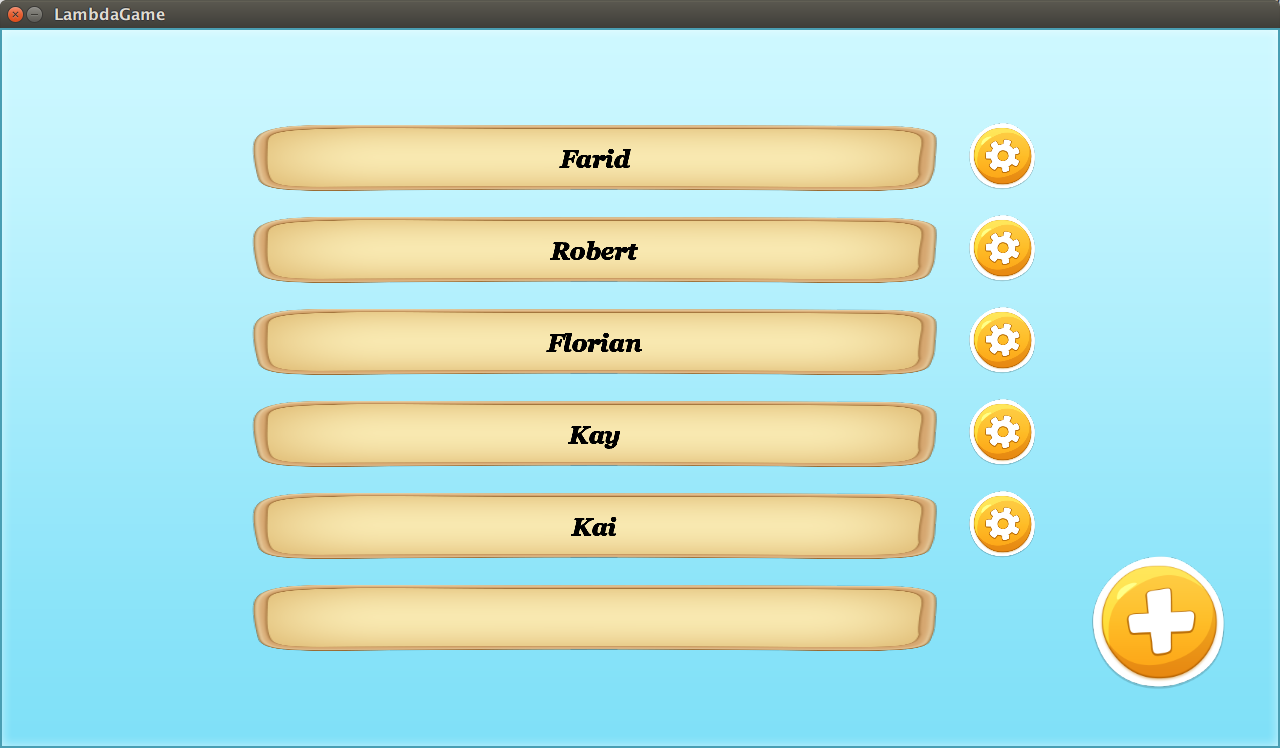
\includegraphics[width=\textwidth]{pictures/profileselection}
\end{frame}

\begin{frame}
	\frametitle{Löschen und Konfigurieren von Profilen}
	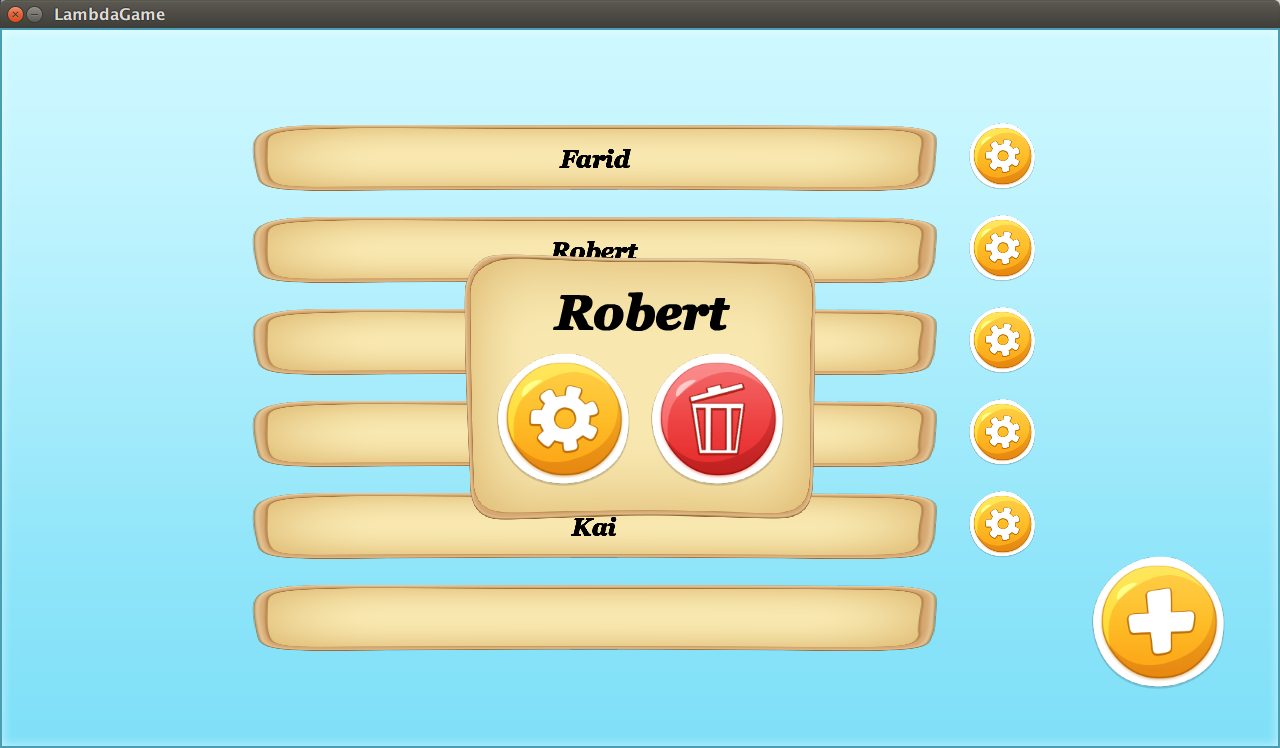
\includegraphics[width=\textwidth]{pictures/profileselection_dialog}
\end{frame}

\begin{frame}
	\frametitle{Auswahl der Sprache}
	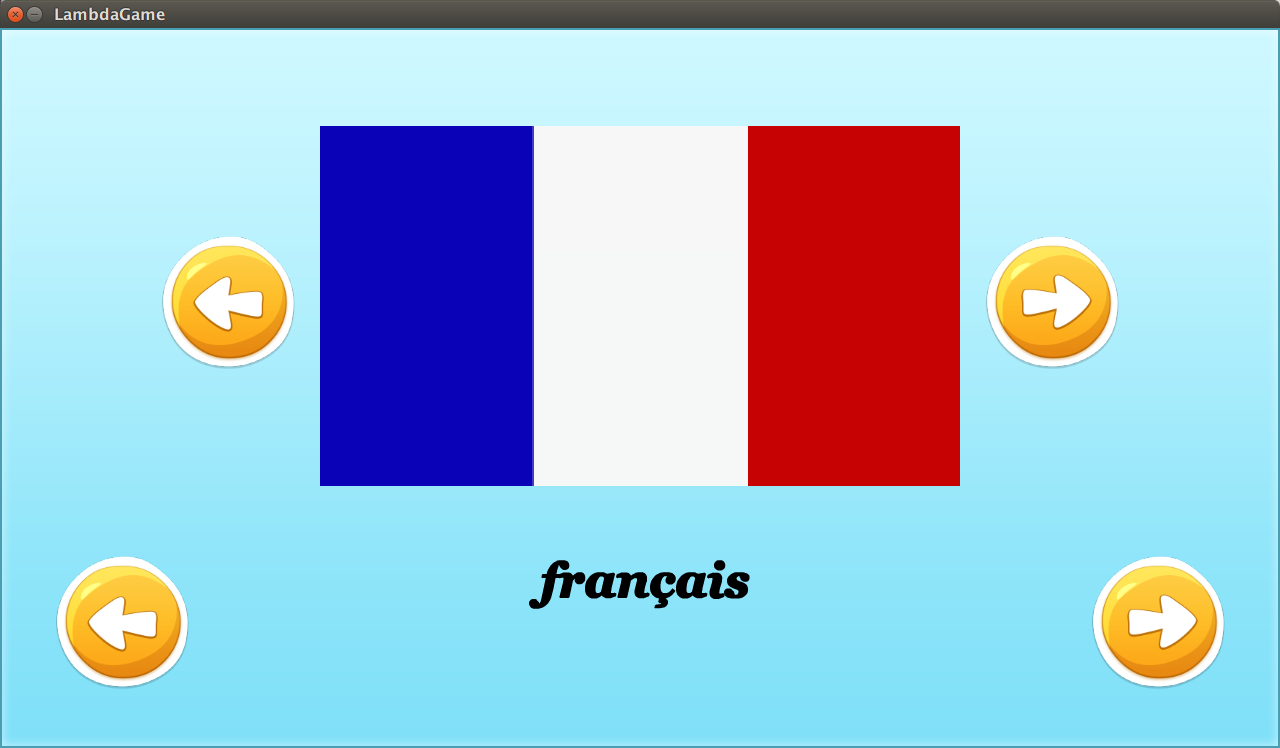
\includegraphics[width=\textwidth]{pictures/languageselection}
\end{frame}

\begin{frame}
	\frametitle{Eingabe des Namens}
	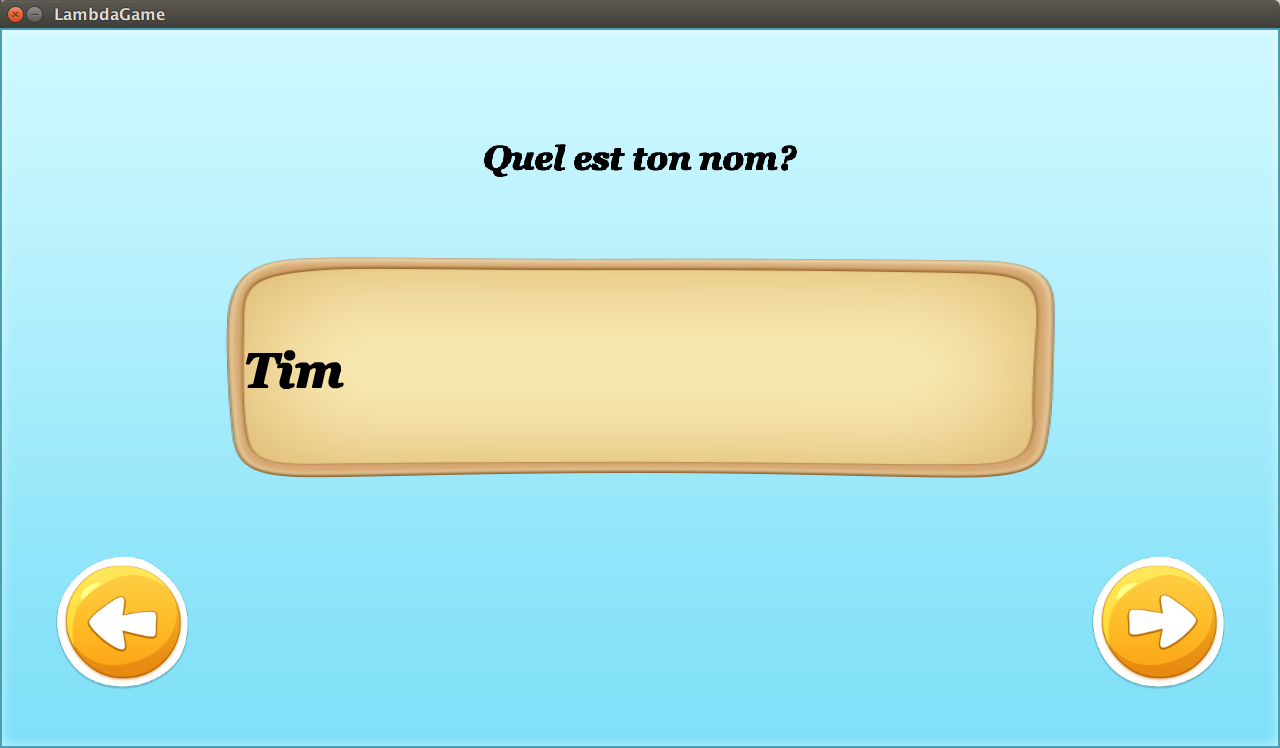
\includegraphics[width=\textwidth]{pictures/nameselection}
\end{frame}

\begin{frame}
	\frametitle{Avatarauswahl}
	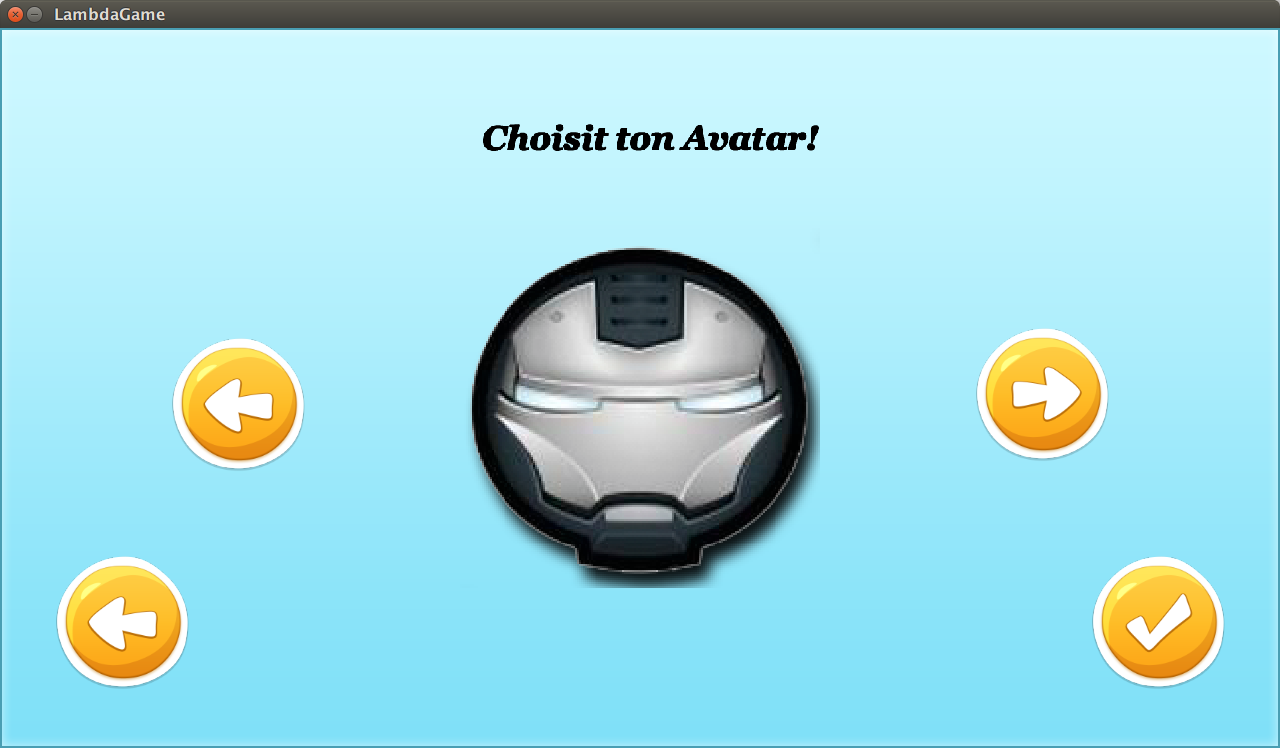
\includegraphics[width=\textwidth]{pictures/avatarselection}
\end{frame}

\begin{frame}
	\frametitle{Verfolgen des Lernfortschritts}
	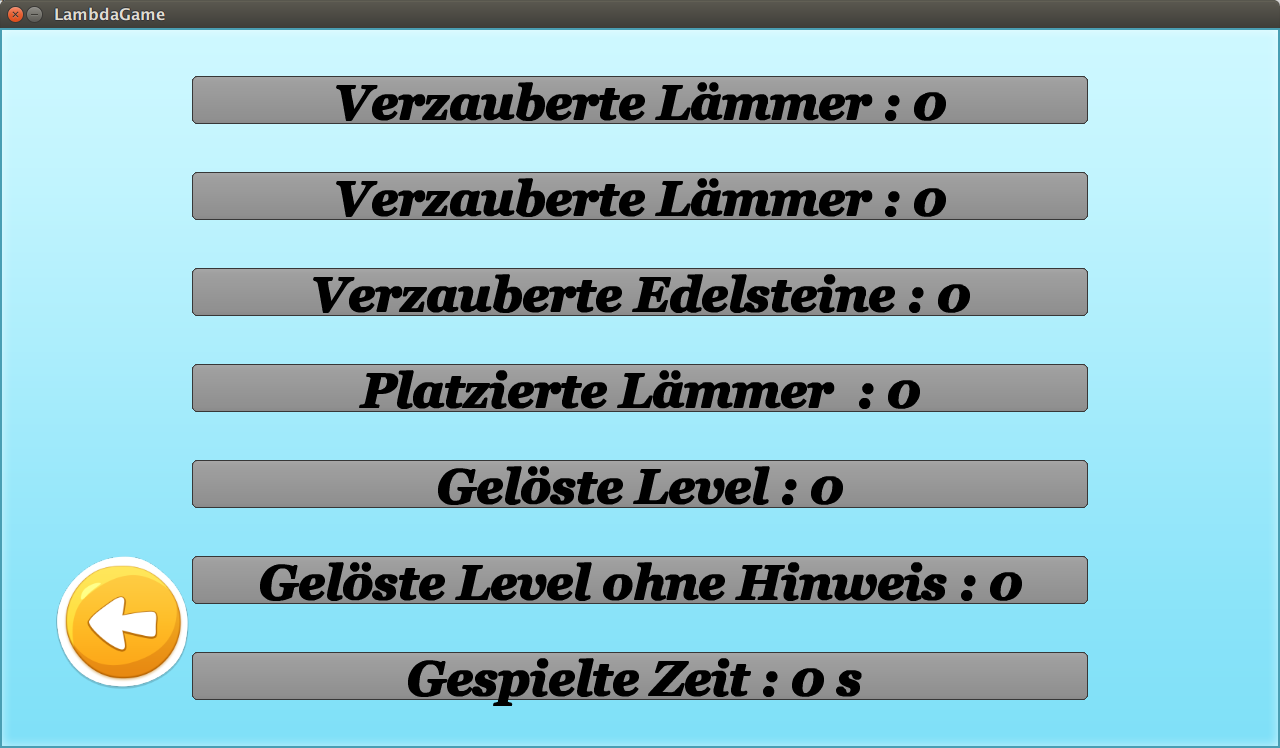
\includegraphics[width=\textwidth]{pictures/statisticmenu}
\end{frame}

\begin{frame}
	\frametitle{Erhaltung der Langzeitmotivation}
	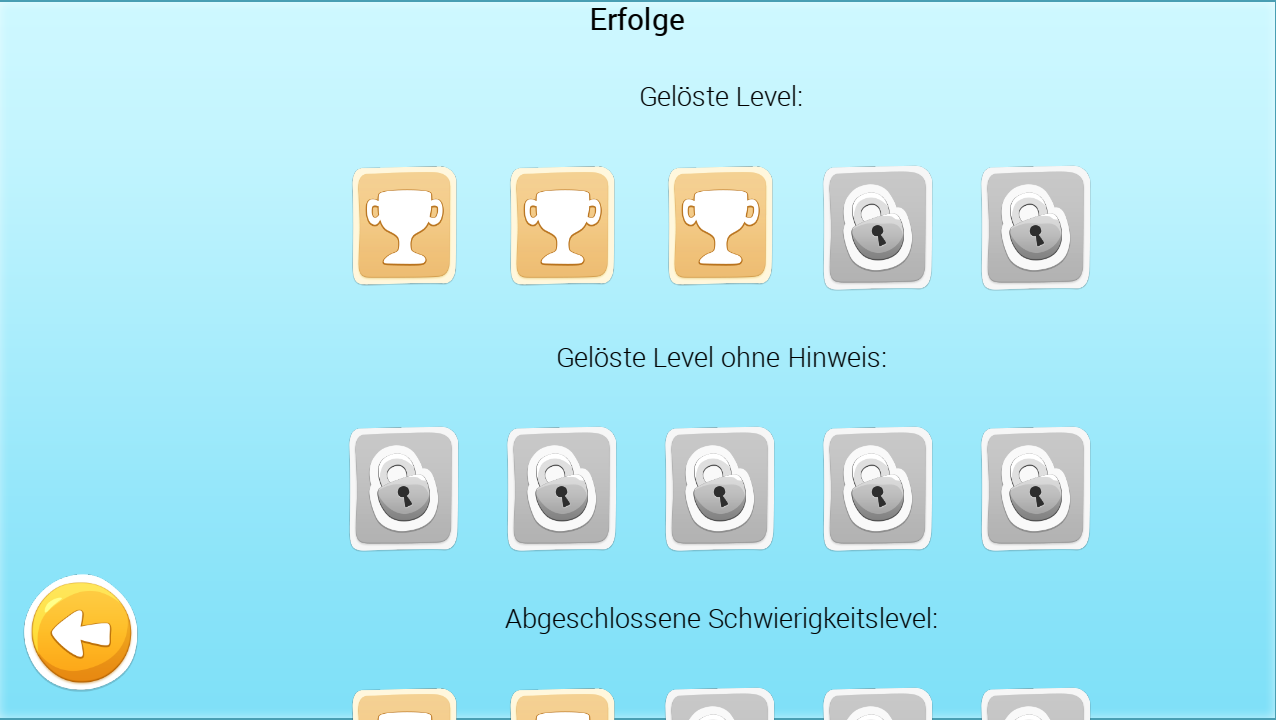
\includegraphics[width=\textwidth]{pictures/achievementvs}
\end{frame}

\begin{frame}[c]
	\begin{center}
	\Huge
	Umgesetzte Wunschkriterien
	\end{center}
\end{frame}

\begin{frame}
	\frametitle{In-Game-Shop}
	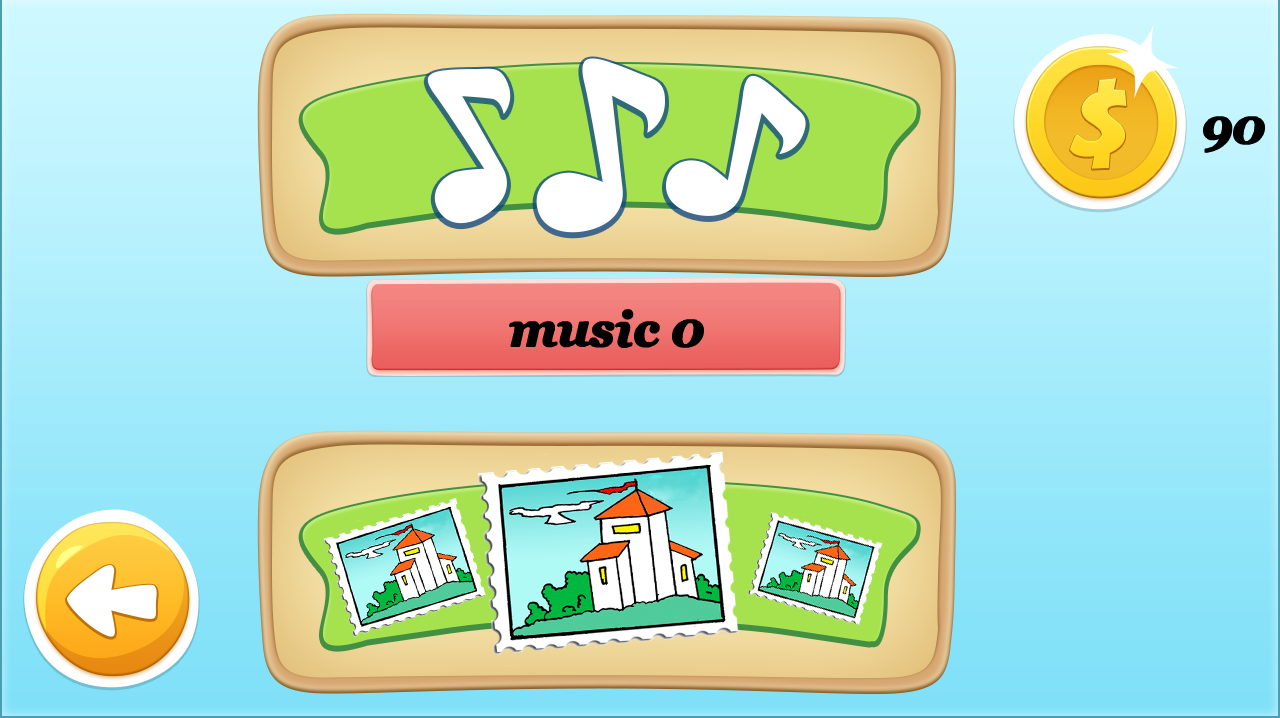
\includegraphics[width=\textwidth]{pictures/shop}
\end{frame}

\begin{frame}
	\frametitle{Sandbox}
	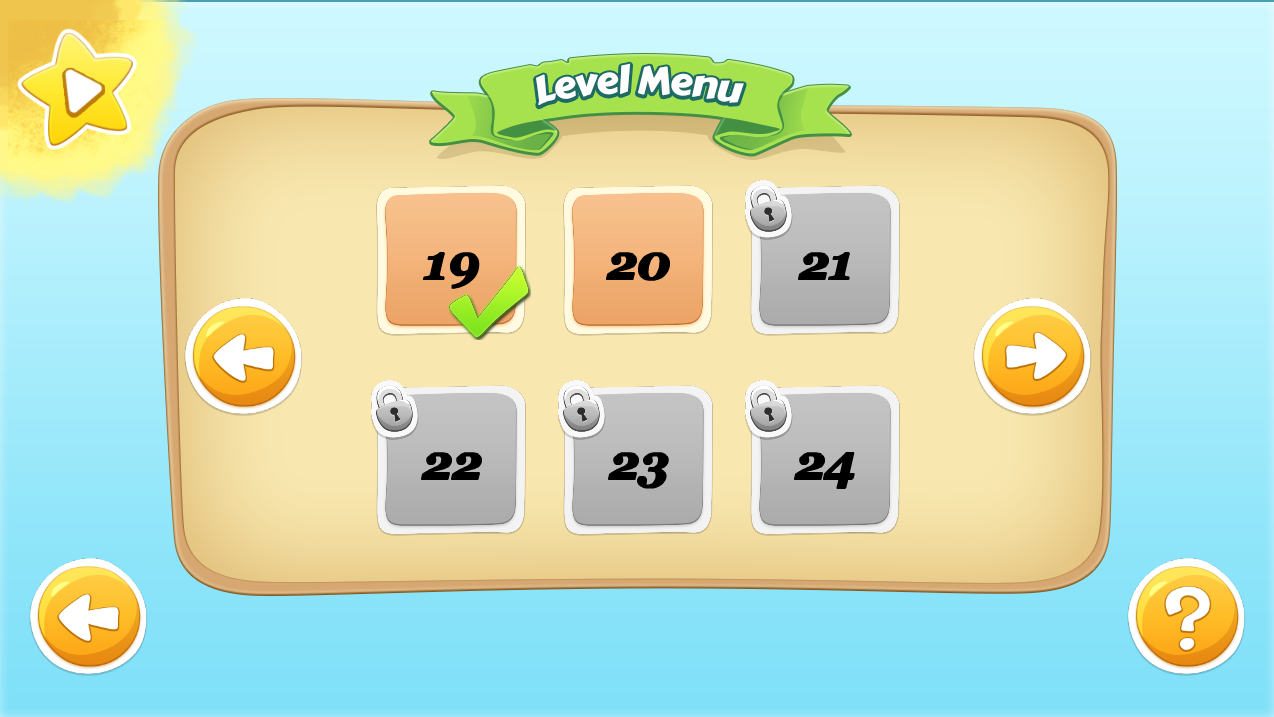
\includegraphics[width=\textwidth]{pictures/levelselectionmenu}
\end{frame}

\begin{frame}
	\frametitle{Hinweise zum Lösen des Levels}
	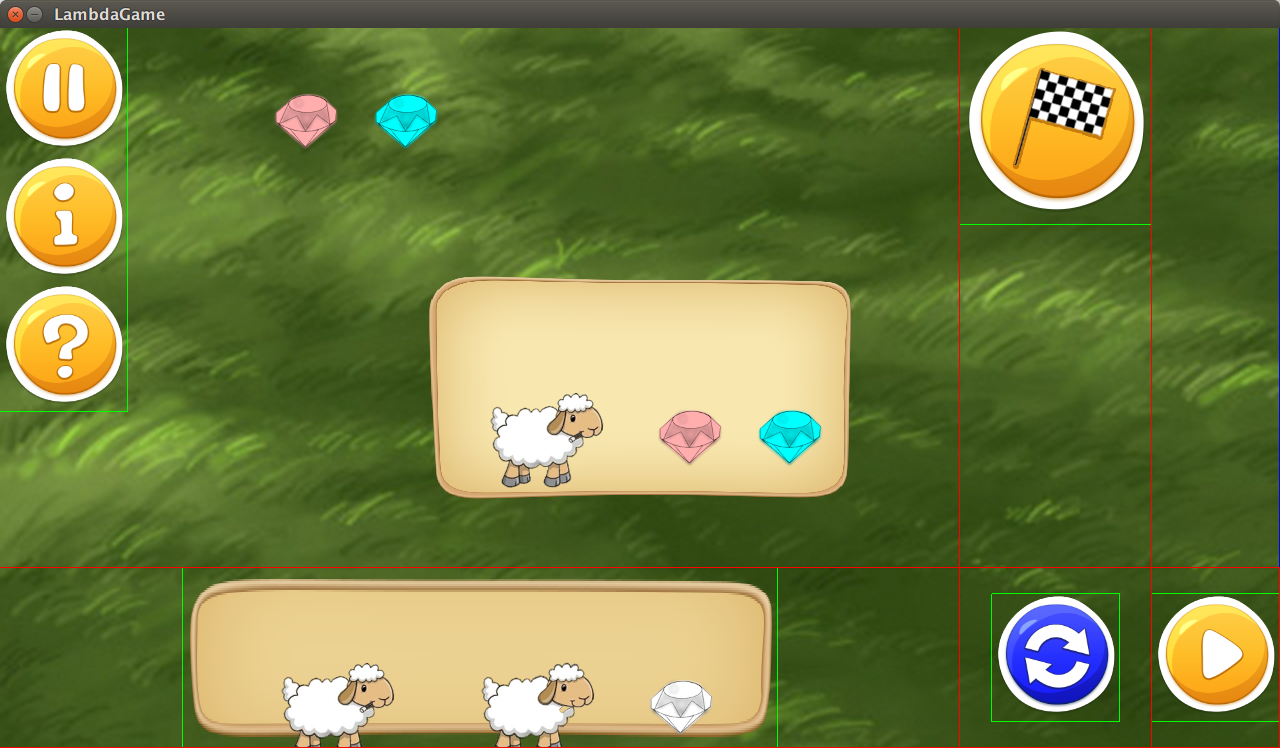
\includegraphics[width=\textwidth]{pictures/hintbutton}
\end{frame}

\begin{frame}
	\frametitle{Unterschiedliche Reduktionsstrategien}
	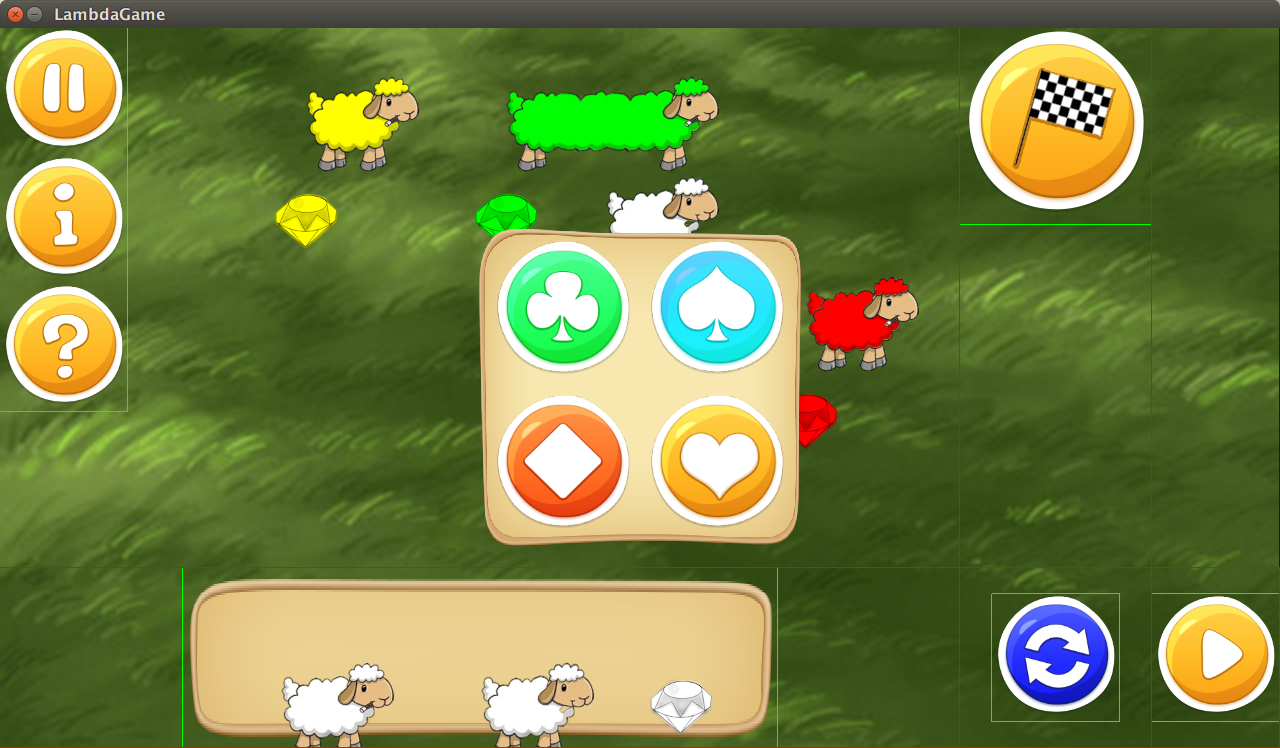
\includegraphics[width=\textwidth]{pictures/reduction_strategies}
\end{frame}

\begin{frame}
	\frametitle{Weitere umgesetzte Wunschkriterien}
	\begin{itemize}[<+->]
		\item Support von weiteren Sprachen
		\begin{itemize}
			\item Englisch
			\item Französisch
		\end{itemize}
		\item Desktop-Version
		\begin{itemize}
			\item Für Windows
			\item Für Mac OS X
		\end{itemize}
		\item Für Tablets angepasste Version
	\end{itemize}
\end{frame}

\begin{frame}
	\frametitle{Gestrichene Wunschkriterien}
	\begin{itemize}[<+->]
		\item Lehrermodus
		\item Farbenblindenmodus
		\item Vermittlung einer Hintergrundgeschichte durch Animationen
	\end{itemize}
\end{frame}

\begin{frame}
	\frametitle{Änderungen am Entwurf}
	\begin{itemize}[<+->]
		\item Keine $\lambda$-Ausdrücke
		\item Neue Struktur zum Laden von Assets
		\begin{itemize}
			\item queueAssets(AssetManager manager)
			\item create(AssetManager manager)
		\end{itemize}
		\item ``Zwischenoberklasse'' StageViewController 
		\item Viele kleine Änderungen
		\begin{itemize}
			\item Fehlerhafte Konstruktoren
			\item Weitere Methoden erforderlich
			\item ...
		\end{itemize}
		\item Keine gravierenden Abweichungen zum Entwurf
	\end{itemize}
\end{frame}

\begin{frame}
	\frametitle{Zeitplan}
	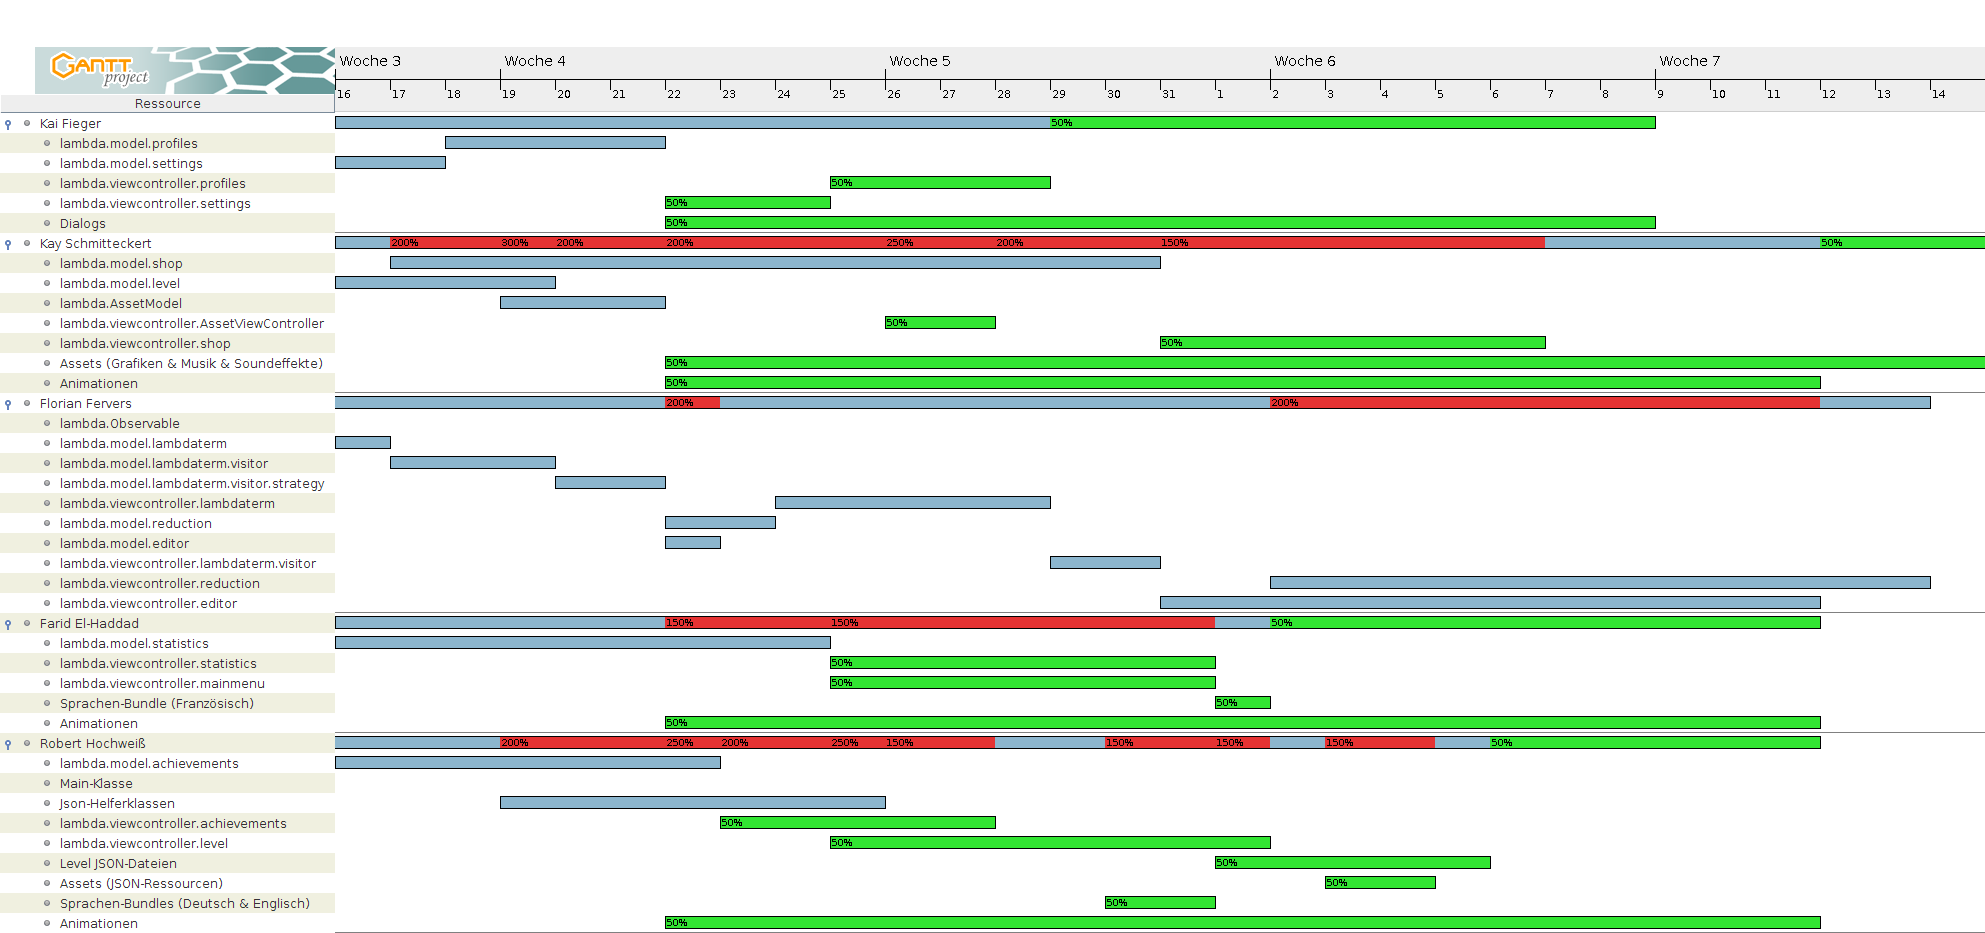
\includegraphics[width=\textwidth]{pictures/Implementierungsplan_ende}
\end{frame}

\begin{frame}
	\frametitle{Statistiken}
	\begin{itemize}[<+->]
		\item 249 Commits
		\item Für die Applikation: 8764 Lines of Code
		\item 26 Packages
		\item 13 Interfaces
		\item 134 Klassen
		\begin{itemize}
			\item 348 Attribute
			\item 733 Methoden
		\end{itemize}
	\end{itemize}
\end{frame}

\begin{frame}
	\centering
	\huge Vielen Dank für Ihre Aufmerksamkeit!
	
\includegraphics[scale=0.8]{team_lambda_lg.png}
\end{frame}

\end{document}
